\documentclass[10pt,a5paper,titlepage,oneside]{book}
%\documentclass{article} % Specifies the document class
%\usepackage[cp1251]{inputenc}


\usepackage[T1,T2A]{fontenc}
\usepackage[utf8]{inputenc}


%\usepackage[T1,T2A]{fontenc}
%\usepackage[cp1251]{inputenc}


\usepackage[intlimits,sumlimits]{amsmath}

\usepackage{enumerate,graphicx,dcolumn,amsthm}
\usepackage[english,ukrainian]{babel}
\usepackage{indentfirst}
\usepackage{caption}[2013/01/20]
%\captionsetup{labelsep=period,font=sf, labelfont=bf, format=plain, justification=centerlast, tablename=Таблиця}
\captionsetup{labelsep=period,font=sf, labelfont=bf, format=plain, justification=justified, tablename=Таблиця, tablewithin=none}

\usepackage{graphicx}
\graphicspath{{Fig/}}
\usepackage{floatflt}
\usepackage{wrapfig}
\usepackage{afterpage}

\usepackage{tabularx}
\renewcommand{\tabularxcolumn}[1]{m{#1}}
\usepackage{hhline}
\usepackage{multirow}
\usepackage{tabu}

\usepackage{longtable}
\usepackage{colortbl}
\definecolor{MyGray}{gray}{0.9}
\doublerulesepcolor[rgb]{1,1,1}

\usepackage{tikz}
\usetikzlibrary{calc}
\usepackage{wrapfig}

 \usepackage[left=20mm,right=15mm,top=15mm,bottom=16mm,bindingoffset=0mm,footskip=6mm,includefoot]{geometry}
\setlength{\parindent}{5mm}
\usepackage[hang,flushmargin]{footmisc}

\pagestyle{plain}



    \usepackage{enumitem}
    \makeatletter
        \AddEnumerateCounter{\asbuk}{\@asbuk}{м)}
    \makeatother
%    \setlist{nolistsep}
%  \setlist{itemindent=0cm,topsep=0cm,parsep=0cm,itemsep=0cm,labelindent=0cm}
   \setlist{nolistsep, topsep=0ex, leftmargin=1ex, itemindent=4ex}
%    \renewcommand{\labelitemi}{$\bullet$}
    \renewcommand{\labelenumi}{\arabic{enumi}.}
    \renewcommand{\labelenumii}{\asbuk{enumii})}



\numberwithin{equation}{part}


\makeatletter


\usepackage {titlesec}
\titleformat{\chapter}{\hyphenpenalty=10000\sf\Large\bfseries}{
\thechapter. }{0pt}{\Large}

\titlespacing*{\chapter}{0pt}{1.1\baselineskip}{\baselineskip}

\titleformat{\section}{\hyphenpenalty=10000\sf\large\bfseries}{
\thesection. }{0pt}{\large}

\makeatother



%\includeonly{
%%title,
%%acronyms,
%%vstup,
%Evolution,
%Swarm,
%Bio,
%Human,
%Physical,
%Math,
%Other,
%Hybrid,
%Multi
%}

\usepackage{pifont}
% Подключаемый Symbol-шрифт,
% Обеспечивает доступность семейства \verb|U/psy/m/n| под именем greek
\DeclareSymbolFont{greek}{U}{psy}{m}{n}
% Выбор команды переключения шрифта
\DeclareSymbolFontAlphabet{\gr}{greek}



\renewcommand{\theequation}{\thechapter.\arabic{equation}}

\usepackage{cite}
\bibliographystyle{utf8gost780u}
%\bibliographystyle{model1-num-names}
%\bibliographystyle{ieeetr}
%\bibliographystyle{acm}

\begin{document}           % End of preamble and beginning of text.

\setcounter{chapter}{1}
\setcounter{section}{1}

\section{Методи до визначення рухливості у кремнії}

Задача оцінки рухливості електронів $\mu_n$ та дірок $\mu_p$ у напівпровіднику 
за певних умов є достатньо поширеною у різноманітних фізичних дослідженнях.
Один з варіантів її вирішення полягає у використанні загального підходу, згідно з яким
\begin{equation}\label{eq1}
  \mu=\frac{e\tau_p}{m_\sigma}\,,
\end{equation}
де
$e$ --- елементарний заряд,
$\tau_p$ --- середній час вільного пробігу носія заряду,
$m_\sigma$ --- ефективна маса електропровідності.

Час вільного пробігу обмежується розсіянням носіїв заряду, яке може бути викликане декількома причинами,
пов'язаними з порушеннями періодичності потенціалу.
Зокрема виділяють розсіяння на коливаннях ґратки (акустичних та оптичних фононах), заряджених та нейтральних домішках,
дислокаціях, границях зерен та інших неоднорідностях структури, поверхнях та межах розділу, інших носіях.
Кожен із цих механізмів має свою залежність від температури, рівня легування та розміру напівпровідникової структури
і може бути визначальним для величини рухливості за певних умов.
Проте найчастіше необхідно враховувати декілька можливих шляхів розсіяння носіїв заряду.
В такому випадку для оцінки рухливості використовується правило Матіссена:
\begin{equation}\label{eq2}
  \mu^{-1}=\sum_i \mu_i^{-1}\,,
\end{equation}
де 
сумування відбувається за механізмами розсіяння,
$\mu_i$ --- рухливість носіїв за наявності лише $i$-го механізму розсіяння. 
Для оцінки $\mu_i$ можна використовувати вирази, аналогічні формулі (\ref{eq1}), розрахувавши відповідний час вільного пробігу.

Для переважної більшості механізмів розсіяння вирази для оцінки рухливості відомі.
Так, при розсіянні на іонізованих домішках нерідко використовується вираз Брукса-Херрінга


%\begin{titlepage}
\begin{center}

{\small Київський національний університет  імені Тараса Шевченка}

{\small фізичний факультет}


\vspace*{2cm}
{\scshape\bfseries\Large О.Я.~ОЛІХ}

\vspace*{1cm}
{\scshape\bfseries\huge методи дослідження дефектів}

\vspace*{0.5cm}
методичний посібник для студентів фізичного факультету

\end{center}
%
%%\vspace*{1cm}
\begin{figure}[h]\center
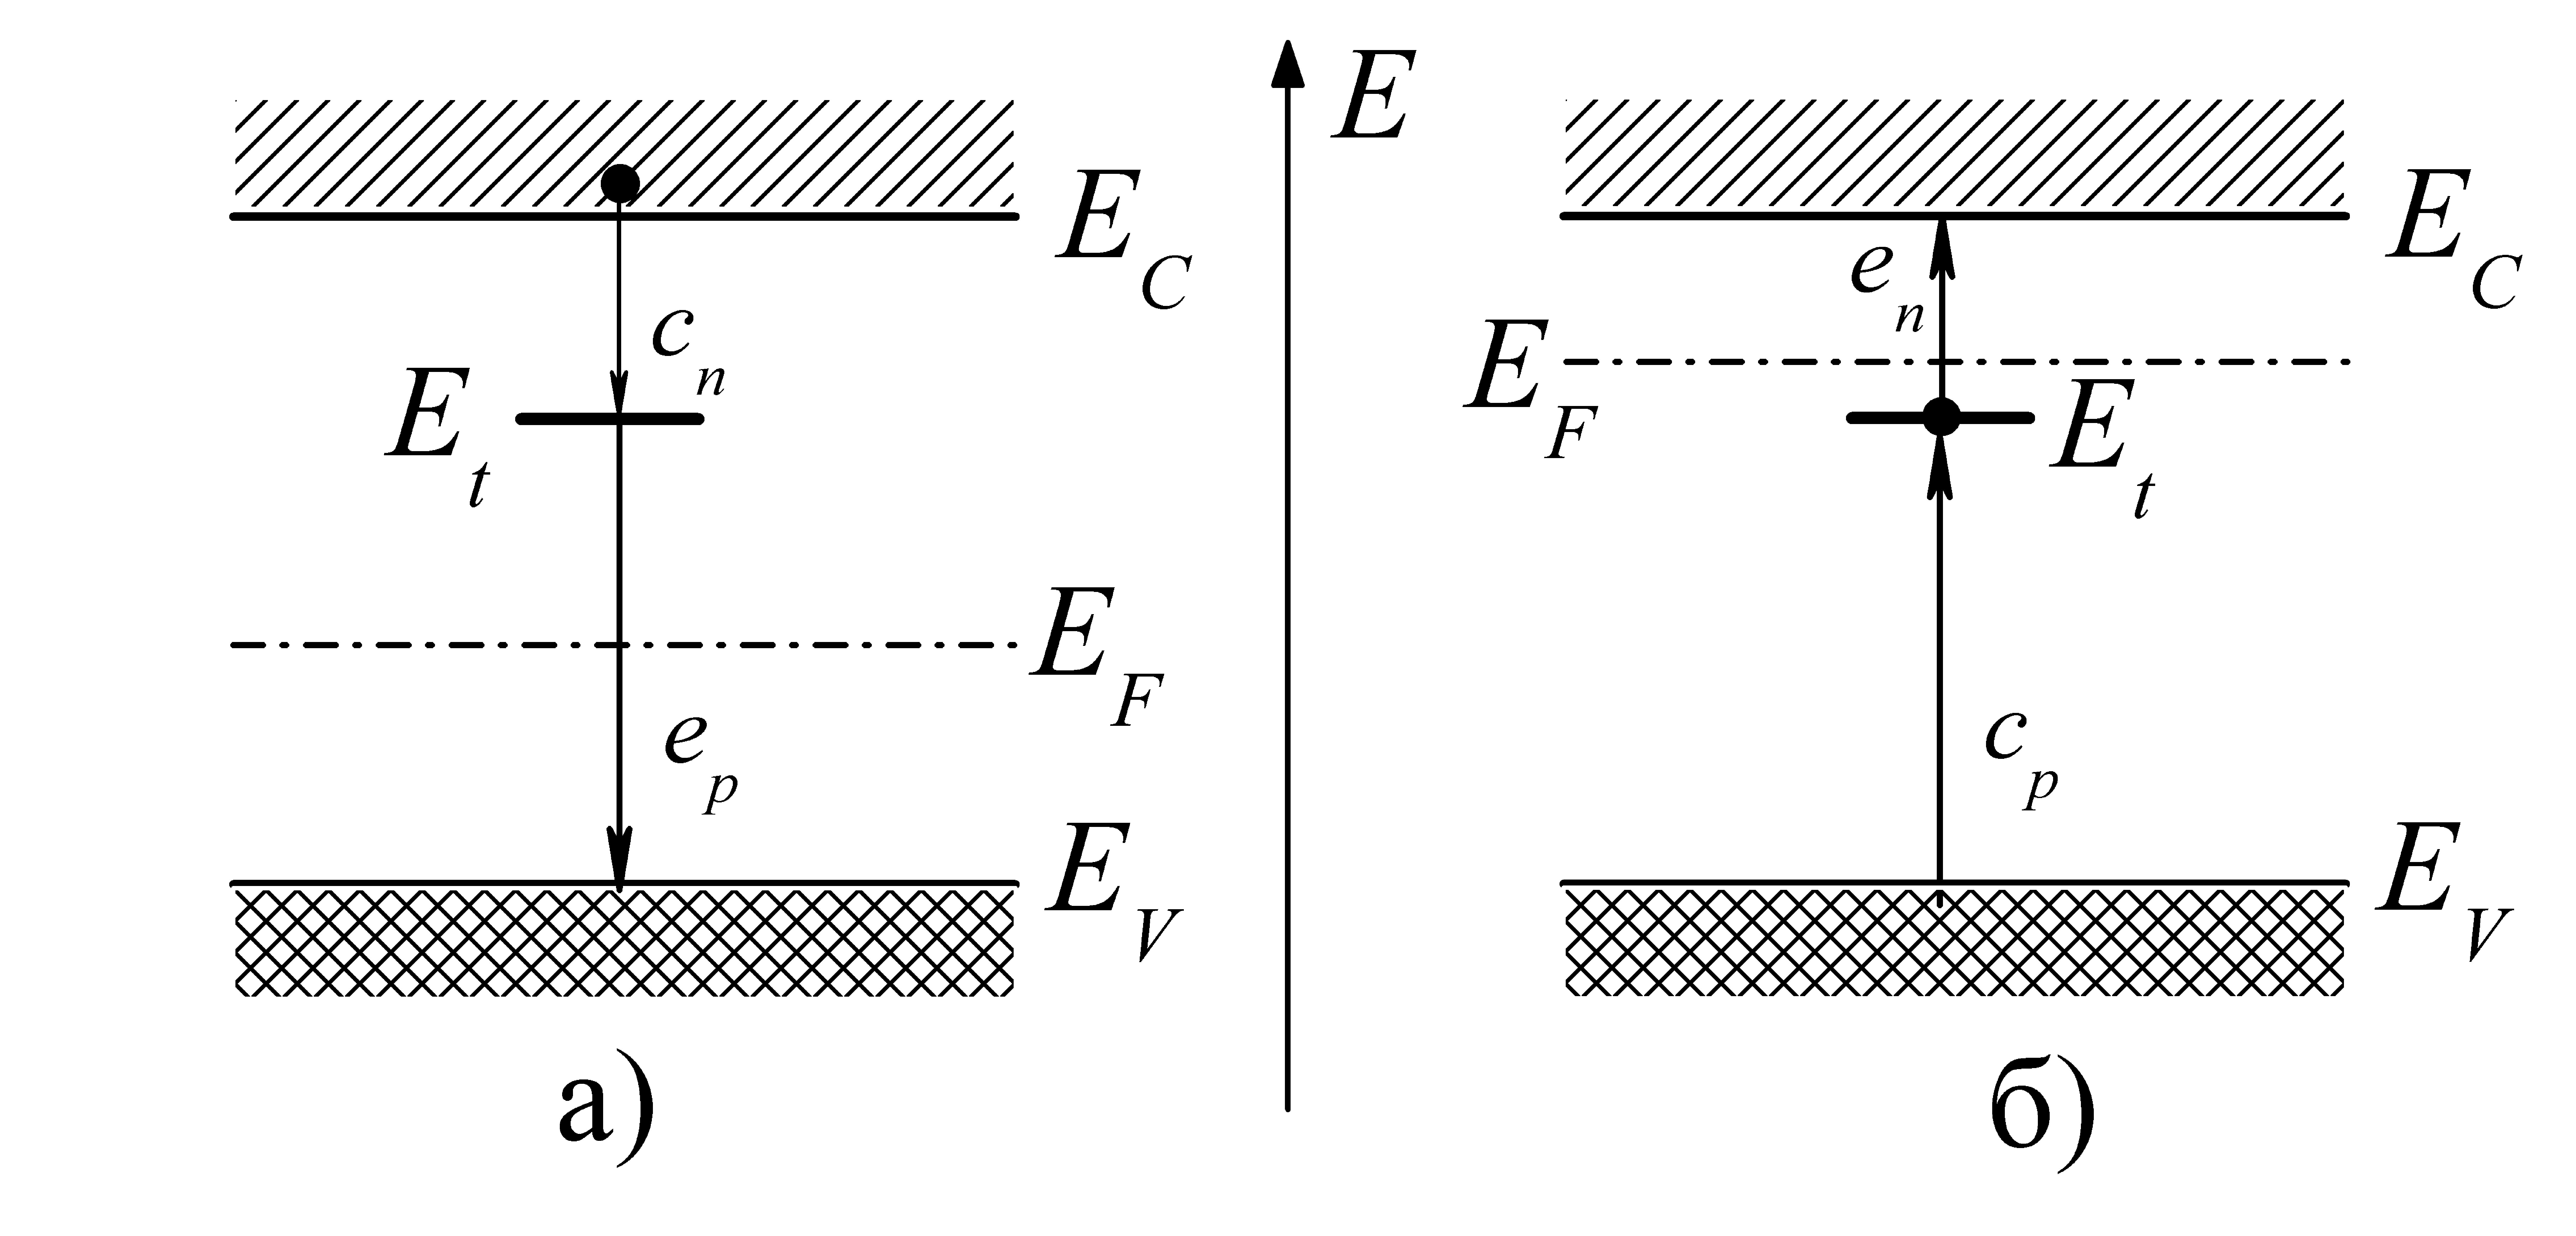
\includegraphics[width=0.4\textwidth]{Fig1_1}
\end{figure}
%
%
\begin{center}

{\scshape\bfseries Київ -- 2020}
\end{center}
\end{titlepage}
Б

УДК 004.7; 004.057.4.

\begin{center}

 \vspace{0.04\textheight}
 Рецензенти:
\end{center}
%\vspace{0.5cm}

\emph{С.В.~Кондратенко}, д-р. фіз.-мат. н., проф.

\emph{О.О.~Коротченков}, д-р. фіз.-мат. н., проф.

\vspace{1cm}
Рекомендовано до друку вченою радою фізичного факультету
Київського національного університету імені Тараса Шевченка
(протокол №10 від 18 квітня 2020 року)



\vspace{1cm}
\textbf{Оліх О.Я.}

Методи дослідження дефектів. Методичний посібник для студентів фізичного факультету. --- К.:2020.
%Іл.~236, табл.~51.

\vspace{1cm}
У посібнику розглянуто основні типи точкових дефектів, методи їх опису та термодинамічні підходи оцінки рівноважної концентрації.
Докладно викладено питання, які стосуються механізмів дифузії точкових дефектів.
Проаналізовано шляхи впливу на дефектну підсистему кристалів радіаційного опромінення і термічної обробки.
Наведено приклади найпоширеніших точкових комплексів у кремнії, а також розглянуто особливості метастабільних та бістабільних дефектів і центрів з від’ємною кореляційною енергією. Посібник містить задачі для самостійного розв’язання. 


%\renewcommand{\theequation}{\thepart.\arabic{equation}}
%\renewcommand\bibname{Рекомендована та використана література}

%\renewcommand{\thesection}{\arabic{chapter}.\arabic{section}.}
\vspace{-5cm}
\setcounter{page}{3}

%\clearpage
%%{\footnotesize
% \tableofcontents
% %}

%\renewcommand{\thesection}{\arabic{section}.}
%\clearpage
%\normalsize




%\addcontentsline{toc}{chapter}{\bibname}
\bibliography{olikh}


\end{document}
